\documentclass[pdftex,12pt,a4paper]{report}

\usepackage[pdftex]{graphicx}
\usepackage[colorlinks=true,
            linkcolor=red,
            citecolor=red]{hyperref}
\usepackage[all]{hypcap}

\newcommand{\HRule}{\rule{\linewidth}{0.5mm}}

\renewcommand{\thesection}{\arabic{section}}
\begin{document}

\renewcommand{\bibname}{References}
%%%%%%%%%%%%%%%%%%%%%%%%%%%%%%%%%%%%%%%%%%%%%%%%%%%%%%%%%%%%%%%%%%%%%%%%%%%%%%%
%%%%%%%%%%%%%%%%%%%%%%%%%%%%%%%%%%%%%%%%%%%%%%%%%%%%%%%%%%%%%%%%%%%%%%%%%%%%%%%
%%%%%%%%%%%%%%%%%%%%%%%%%%%%%%%%%%%%%%%%%%%%%%%%%%%%%%%%%%%%%%%%%%%%%%%%%%%%%%%

\begin{titlepage}
\begin{center}

% Upper part of the page. The '~' is needed because \\
% only works if a paragraph has started.

\includegraphics[width=0.3\textwidth]{./res/hku-logo}~\\[1cm]

% \textsc{\LARGE The University of Hong Kong}\\[0.5cm]
% \textsc{\LARGE Faculty of Engineering}\\[0.5cm]
% \textsc{\LARGE Department of Computer Science}\\[1.5cm]
\uppercase{\LARGE The University of Hong Kong}\\[0.5cm]
\uppercase{\LARGE Faculty of Engineering}\\[0.5cm]
\uppercase{\LARGE Department of Computer Science}\\[1.5cm]

% \textsc{\Large Final Year Project}\\[0.5cm]
\uppercase{\Large Final Year Project}\\[0.5cm]

% Title
\HRule \\[0.4cm]
{ \huge \bfseries Person Identification from Images and Videos \\[0.4cm] }

\HRule \\[1.5cm]

% Author and supervisor
\begin{minipage}{0.4\textwidth}
\begin{flushleft} \large
\emph{Author:}\\
Sai \textsc{Bi} (2011810096)
\end{flushleft}
\end{minipage}
\begin{minipage}{0.4\textwidth}
\begin{flushright} \large
\emph{Supervisor:} \\
Prof. Yizhou \textsc{Yu}
\end{flushright}
\end{minipage}

\vfill

% Bottom of the page
{\large \today}

\end{center}
\end{titlepage}

%%%%%%%%%%%%%%%%%%%%%%%%%%%%%%%%%%%%%%%%%%%%%%%%%%%%%%%%%%%%%%%%%%%%%%%%%%%%%%%
%%%%%%%%%%%%%%%%%%%%%%%%%%%%%%%%%%%%%%%%%%%%%%%%%%%%%%%%%%%%%%%%%%%%%%%%%%%%%%%
%%%%%%%%%%%%%%%%%%%%%%%%%%%%%%%%%%%%%%%%%%%%%%%%%%%%%%%%%%%%%%%%%%%%%%%%%%%%%%%
\hypersetup{
     colorlinks=true,
     linkcolor=black, 
     citecolor=red
}
\tableofcontents


\hypersetup{
     colorlinks=true,
     linkcolor=red, 
     citecolor=red
}
%%%%%%%%%%%%%%%%%%%%%%%%%%%%%%%%%%%%%%%%%%%%%%%%%%%%%%%%%%%%%%%%%%%%%%%%%%%%%%%
%%%%%%%%%%%%%%%%%%%%%%%%%%%%%%%%%%%%%%%%%%%%%%%%%%%%%%%%%%%%%%%%%%%%%%%%%%%%%%%
%%%%%%%%%%%%%%%%%%%%%%%%%%%%%%%%%%%%%%%%%%%%%%%%%%%%%%%%%%%%%%%%%%%%%%%%%%%%%%%
\chapter*{Project plan}
\addcontentsline{toc}{chapter}{Project plan}
\section{Person identification}\index{Introduction}
Person identification is the process of identifying or verifying a person from 
a digital image or video frame from a video source. With increasing number of
surveillance cameras installed in public area and automatic identification
widely used in industry as well as government especially for law enforcement and
security purpose, it is essential to find more accurate and efficient
algorithms to this problem. In our project, we are going to explore new 
approaches for person identification with face information and body information.


\begin{figure}[b]
    \begin{center}
        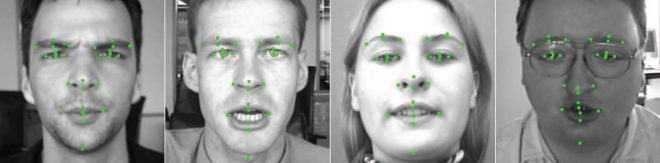
\includegraphics[width=0.8\textwidth]{./res/facekeypoint}
    \end{center}
    \caption{Examples of face keypoints}
    \label{fig:facekeypoint}
\end{figure}



\subsection{Face-based person identification} \index{Face-based person
identification}
For this approach, we capture each individual's face images, and identify a
person through face recognition. Multiple methods have been developed for face
recognition, such as principle component analysis(PCA) using eigenfaces, linear
discriminate analysis. Such a problem becomes challenging when face images are
taken with extreme poses, lightings, expressions, and occlusions. Therefore, it
is often necessary to do face alignment before recognition with the help of face
key points such as eye corners, mouth corners, and nose
tip(Figure~\ref{fig:facekeypoint}). The performance of
a face recognition system is to a large degree dependent on the accuracy of face
keypoint detection. Consequently, it is meaning full to find better methods for
face keypoint detection, which is also our focus in order to improve the
accuracy of face recognition.

\subsection{Body-based person identification} \index{Body-based person
identification}
For many applications such as person tracking or person retrieval, it is not
necessary to uniquely identify a person. It often suffices to determine previous 
or future occurrences of the same person in other images or videos. It can find 
applications in modern surveillance systems, either for online tracking of an 
individual over a network of cameras or offline retrieval of all videos 
containing a person of interest. 

\begin{figure}[h]
    \begin{center}
        \includegraphics[width=0.8\textwidth]{./res/personreiden}
    \end{center}
    \caption{Sample images for body-based person identification. Images on the
    same column belong to the same person.}
    \label{fig:personreiden}
\end{figure}

This problem is more challenging because when matching images of the same person 
captured with non-overlapping cameras, there 
may exist huge discrepancies in terms of human poses, illumination, camera views 
and photometric settings, and so on(Figure~\ref{fig:personreiden}). In addition, 
the lack of sufficient 
resolution in surveillance cameras makes it infeasible to identify a person 
using face verification. In this case, a total different method from that for 
face recognition is needed.

\section{Objective}\index{Objective}
This project aims to explore new approaches for face-based and body-based person
identification, and improve its accuracy. In particularly, for face-based person
identification, our focus is on developing new methods for more accurate face
keypoints detection.
Based on the new approach, we expect
to develop an integrated system for person identification, covering the process
from photo taking, image cropping, feature extraction, to identification.

\section{Related work}\index{Related work}
There are two major approaches to body-based person identification, namely unsupervised 
matching of image features~\cite{unsupervised_1, unsupervised_2,unsupervised_3} 
and training a decision function to assess the similarity of features in two
images~\cite{article_5,article_6,article_10}. 
These two approaches are developed for different application scenarios. The 
unsupervised approach is better suited for scenarios where it is impractical 
to obtain training images that capture the same group of people from all cameras 
involved. However, whenever such training images can be obtained, the second 
supervised approach is more appropriate since it typically achieves a better 
performance.

Most face alignment approaches can also be classified into two categories,
optimization-based~\cite{Matthews03activeappearance,saragih_goecke2007} and
regression-based~\cite{Cristinacce_boostedregression,so75978}. 
The former one learns face models by
minimizing an self-defined error functions which estimates the alignment error,
and its accuracy depends on the the goodness of error functions and whether they
can be optimized well. The latter one learns a regression function that directly
maps image appearance to the target output, and the complex variations of faces
are learnt from large training data and testing is usually efficient.

%%%%%%%%%%%%%%%%%%%%%%%%%%%%%%%%%%%%%%%%%%%%%%%%%%%%%%%%%%%%%%%%%%%%%%%%%%%%%%%
%%%%%%%%%%%%%%%%%%%%%%%%%%%%%%%%%%%%%%%%%%%%%%%%%%%%%%%%%%%%%%%%%%%%%%%%%%%%%%%
%%%%%%%%%%%%%%%%%%%%%%%%%%%%%%%%%%%%%%%%%%%%%%%%%%%%%%%%%%%%%%%%%%%%%%%%%%%%%%%
\section{Methodology}\index{Methodology}
\subsection{Mutiple experts for body-based person identification}\index{Mutiple 
experts for body-based person identification}
We have noticed that highly discriminative feature descriptors such as local
binary patterns(LBP) and color historgrams are critical to achieve high
accuracy, and these feature descriptors are often of high dimensional. High 
dimensional features are necessary to high performance, but they also introduce
the extra problems like overfitting and large amount of computations. Therefore,
dimension reduction methods such as PCA and CCA are often applied to 
aggressively reduce the dimension of feature descriptors. However, in this 
process subtle but highly discriminative information may be overlooked, 
especially when many different types of features are combined together, which 
decreases the discriminative power of the new features after dimension reduction.

Considering this, our solution is inspired by the behavior of human witnesses. 
Imagine multiple witnesses work together in an effort to reenact a past event 
and draw conclusions. Suppose none of them saw the complete event. Each of them 
would try to recall the partial evidences he/she has and provide opinions 
accordingly. At the end, a much more complete understanding of the event as 
well as some conclusions can be reached by piecing together the partial 
evidences and opinions from individual witnesses. In the same spirit, we 
hope to propose a method that trains a group of witness functions, 
each of which is only exposed to a random subset of the input features. Each 
witness function produces an opinion according to the partial features it has. 
We will aslo introduce a weighted fusion scheme to combine the opinions of multiple 
witness functions together.

\subsection{Regression with neural network for face keypoints detection}


\section{Timeline}\index{Timeline}
\begin{table}[t]
    \begin{tabular}{|l|l|}
    \hline
    Oct 20th, 2013 & Design of algorithms for body-based person identification \\ \hline
    Nov 30th, 2013 & Algorithm implementation \\ \hline
    Jan 14th, 2013 & Testing and further adjustion \\ \hline
    Jan 16th, 2014 & First presentation  \\ \hline
    Jan 26th, 2014 & Detailed intermediate report \\ \hline
    Feb 10th, 2014 & Design of algorithms for face keypoints detection \\ \hline
    Feb 20th, 2014 & Algorithm implementation \\ \hline
    Mar 28th, 2014 & Testing and further adjustion \\ \hline 
    Apr 20th, 2014 & Final presentation and final report \\  \hline
    May 4th, 2014 & Project exhibation \\ \hline
    \end{tabular} 
    \caption{Timeline}
\end{table}








\cleardoublepage
\phantomsection
\addcontentsline{toc}{chapter}{References}
\bibliographystyle{plain}
\bibliography{proposal}

\end{document}
